\documentclass[12pt,a4paper]{article}
\usepackage{amsmath,amsthm,amsfonts,amssymb,amscd}
\usepackage{times}              
% Use Times New Roman
\usepackage{graphicx}           
% Enhanced support for images
\usepackage{float}              
% Improved interface for floating objects
\usepackage{booktabs}           
% Publication quality tables
\usepackage{xcolor}             
% Driver-independent color extensions
\usepackage{geometry}           
% Customize document dimensions
\usepackage{fullpage}           
% all 4 margins to be either 1 inch or 1.5 cm
\usepackage{comment}            
% Commenting
\usepackage{minted}             
% Highlighted source code. Syntax highlighting
\usepackage{listings}           
% Typeset programs (programming code) within LaTeX
\usepackage{lastpage}           
% Reference last page for Page N of M type footers.
\usepackage{fancyhdr}           
% Control of page headers and footers
\usepackage{hyperref}           
% Cross-referencing 
\usepackage[small,bf]{caption}  
% Captions
\usepackage{multicol}
\usepackage{tikz}               
% Creating graphic elements
\usepackage{circuitikz}         
% Creating circuits
\usepackage{verbatim}          
% Print exactly what you type in
\usepackage{cite}               
% Citation
\usepackage[us]{datetime} 
% Various time format
\usepackage{blindtext}
% Generate blind text
\usepackage[utf8]{inputenc}
\usepackage{array}
\usepackage{makecell}
\usepackage{tabularx}
\usepackage{titlesec}
\usepackage{multicol}
\DeclareUnicodeCharacter{2212}{-}


\setlength\parindent{0pt}

%%%%%%%%%%%%%%%%%%%%%%%%%%%%%%%%%%%%%%%%%%%%%%%%%%%%%%%%%%%%%%
\titleformat{\section}
{\color{UM_DarkBlue}\normalfont\large\bfseries}
{\color{UM_DarkBlue}\thesection}{1em}{}

%%%%%%%%%%%%%%%%%%%%%%%%%%%%%%%%%%%%%%%%%%%%%%%%%%%%%%%%%%%%%%
\hypersetup{
    draft=false,
    final=true,
    colorlinks=true,
    citecolor=UM_DarkBlue,
    anchorcolor=yellow,
    linkcolor=UM_DarkBlue,
    urlcolor=UM_DarkBlue,
    filecolor=green,      
    pdfpagemode=FullScreen,
    bookmarksopen=false
    }
    
%%%%%%%%%%%%%%%%%%%%%%%%%%%%%%%%%%%%%%%%%%%%%%%%%%%%%%%%%%%%%%
\lstdefinestyle{Fortran}{
basicstyle=\scriptsize,        % the size of the fonts that are used for the code
  breakatwhitespace=false,         % sets if automatic breaks should only happen at whitespace
  breaklines=false,                 % sets automatic line breaking
  captionpos=b,                    % sets the caption-position to bottom
  commentstyle=\color{mygreen},    % comment style
  extendedchars=true,              % lets you use non-ASCII characters; for 8-bits encodings only, does not work with UTF-8
  keepspaces=true,                 % keeps spaces in text, useful for keeping indentation of code (possibly needs columns=flexible)
  keywordstyle=\color{blue},       % keyword style
  language=[95]Fortran,                 % the language of the code
  numbers=left,                    % where to put the line-numbers; possible values are (none, left, right)
  numbersep=5pt,                   % how far the line-numbers are from the code
  numberstyle=\tiny\color{mygray}, % the style that is used for the line-numbers
  rulecolor=\color{black},         % if not set, the frame-color may be changed on line-breaks within not-black text (e.g. comments (green here))
  showspaces=false,                % show spaces everywhere adding particular underscores; it overrides 'showstringspaces'
  showstringspaces=false,          % underline spaces within strings only
  showtabs=false,                  % show tabs within strings adding particular underscores
  stepnumber=1,                    % the step between two line-numbers. If it's 1, each line will be numbered
  stringstyle=\color{mymauve},     % string literal style
  tabsize=4,                       % sets default tabsize to 2 spaces
  title=\lstname                   % show the filename of files
}

%%%%%%%%%%%%%%%%%%%%%%%%%%%%%%%%%%%%%%%%%%%%%%%%%%%%%%%%%%%%%%%
\definecolor{UM_Brown}{HTML}{0D190D}
\definecolor{UM_DarkBlue}{HTML}{2264B0}
\definecolor{UM_LightBlue}{HTML}{1CA9E1}
\definecolor{UM_Orange}{HTML}{fEB415}




%\newcommand{\tu}[1]{\textup{#1}}
\newcommand{\tu}[1]{\mathrm{#1}}







\newcommand{\ones}{\mathbf 1}
\newcommand{\reals}{{\mbox{\bf R}}}
\newcommand{\integers}{{\mbox{\bf Z}}}
\newcommand{\symm}{{\mbox{\bf S}}}  % symmetric matrices

\newcommand{\nullspace}{{\mathcal N}}
\newcommand{\range}{{\mathcal R}}
\newcommand{\Rank}{\mathop{\bf Rank}}
\newcommand{\Tr}{\mathop{\bf Tr}}
\newcommand{\diag}{\mathop{\bf diag}}
\newcommand{\card}{\mathop{\bf card}}
\newcommand{\rank}{\mathop{\bf rank}}
\newcommand{\conv}{\mathop{\bf conv}}
\newcommand{\prox}{\mathbf{prox}}

\newcommand{\Expect}{\mathop{\bf E{}}}
\newcommand{\Prob}{\mathop{\bf Prob}}
\newcommand{\Co}{{\mathop {\bf Co}}} % convex hull
\newcommand{\dist}{\mathop{\bf dist{}}}
\newcommand{\argmin}{\mathop{\rm argmin}}
\newcommand{\argmax}{\mathop{\rm argmax}}
\newcommand{\epi}{\mathop{\bf epi}} % epigraph
\newcommand{\Vol}{\mathop{\bf vol}}
\newcommand{\dom}{\mathop{\bf dom}} % domain
\newcommand{\intr}{\mathop{\bf int}}
\newcommand{\sign}{\mathop{\bf sign}}

\newcommand{\cf}{{\it cf.}}
\newcommand{\eg}{{\it e.g.}}
\newcommand{\ie}{{\it i.e.}}
\newcommand{\etc}{{\it etc.}}




\begin{document}

   
    \begin{center}
        \textbf{\Large Sofja Wassiljewna Kowalewskaja}\\
        \vspace{5pt}
        \textit{15 January 1850 - 10 February 1891} \\
        \vspace{20pt}
    \end{center}
    
 \begin{flushleft}
        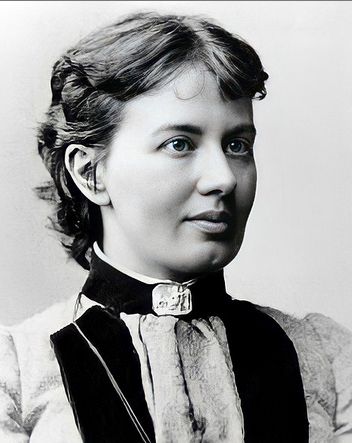
\includegraphics[height=150pt]{images/bios/Kowalewskaja.png}
    \end{flushleft}


%\begin{multicols}{1}


%\section*{}
%\section{First Section}
\vspace{2cm}
Kovalevskaya was the first woman to gain a degree for her contributions to mathematics. She was also known for her literary works and her activism for women's rights. Born Sofia Vasilievna Krukovsky, she was called Sophie, an anglicized version of Sofia. Among her friends, she was known as Sonya or Sonja. Kovalevskaya is the feminine form of her husband's name, Kovalevsky, which is sometimes transliterated as Kovalevskaia or Kovalevskaja.
As a child, Sofja Kolwalewskaja's bedroom walls were wallpapered with her father's mathematics notes from his student days. This was because they had ordered one roll short of wallpaper, and the mathematical notes intrigued her. Born into a minor noble family, she was fortunate enough to receive tutoring in elementary mathematics. Later, she received calculus tutoring from Strannoliubskii, a well-known advocate for women's higher education.


When her older sister met the son of a local priest, Anyuta, inspired by his university studies, decided to go to St. Petersburg to live and proposed living in a commune with young people without servants. However, her father did not allow this, and in response, Anyuta secretly wrote and published two pieces under a male pseudonym. As a woman, Sofja faced limitations in completing her education in Russia. In 1868, she entered a "fictitious marriage" with Vladimir Kovalevskij so they could go to Vienna, where she studied physics while he studied palaeontology.


They spent several months in St. Petersburg studying various subjects before moving to the University of Heidelberg in 1869. She attended physics courses by Hermann von Helmholtz, Gustav Kirchhoff, and Robert Bunsen there. She also studied mathematics with Leo Königsberger and Professor Paul du Bois-Reymond, both Weierstrass students. In 1869, during a trip to London with Vladimir, she attended George Eliot's Sunday salons, where she met Herbert Spencer. This encounter led to a debate on "woman's capacity for abstract thought," which may have inspired a passage in Eliot's novel Middlemarch.


In October 1870, Kovalevskaya moved to Berlin, where she began private lessons with Karl Weierstrass. Weierstrass was often referred to as the "father of modern analysis" and significantly impacted Kovalevskaya's work. They formed a close intellectual and personal relationship beyond the typical teacher-student dynamic. Over eighteen months, she wrote three dissertations under Weierstrass's guidance and presented papers on partial differential equations, the dynamics of Saturn's rings, and elliptic integrals. Her work on partial differential equations included the Cauchy-Kovalevskaya theorem, which proves the existence and uniqueness of local solutions for analytic partial differential equations associated with Cauchy's initial value problems.


In 1878, Sofia and Vladimir had a daughter nicknamed "Foufie." Sofia faced challenges securing a professorship due to her gender, while Vladimir's radical beliefs hindered his career prospects. They tried various schemes to make money. After raising their daughter, Sofia left Vladimir and resumed her work in mathematics. In 1883, she accepted a teaching position at the University of Stockholm, where she became the editor of the mathematics journal Acta Mathematica. She was the first woman to hold this title and received the Prix Bordin award from the French Academy of Science.



Sofia developed a close friendship with Anne Charlotte Edgren-Leffler, the sister of Mittag-Leffler, a mathematician who played a significant role in Sofia's career. Together, they wrote stage plays and a memoir titled "A Russian Childhood." Sofia also wrote "Nihilist Girl" in 1890, a semi-autobiographical account of her life. In June 1889, she became the first woman to hold a chair at a European university since the physicist Laura Bassi in 1750. Tragically, Sofia died from pneumonia at forty-one while returning from a vacation.

%\section{First Section}

%\end{multicols}




%%%%%%%%%%%%%%% REFERENCES %%%%%%%%%%%%%%% 
%\bibliographystyle{IEEEtran}
%\bibliography{References}








\end{document}
